%!TEX root = ../thesis.tex

\chapter{MOOD and MODALITY choices in the Forum} \label{chap:interpersonal}

With an overview of shallow linguistic features in each \gls{corpus}, as well as a basic qualitative understanding of \glspl{post} and their generic properties, the investigation can begin to shift toward individual grammatical systems and the lexical choices at the most delicate end of each system's instantiative cline.

In this chapter, I present findings from an analysis of \sctext{Mood} and \sctext{Modality} choices, which are responsible for making interpersonal meanings---that is, they are used to negotiate the roles and responsibilities of interactants. Frequencies for choices of Mood and Indicative Type are calculated first. This is followed by an account of modalisation, Mood Elements, and brief descriptions of \sctext{tense} and \sctext{polarity} systems.%
\endnote{M\scriptsize{OOD}\footnotesize~structure is not well\hyp{}annotated in most typed dependency grammars currently used for parsing. As such, M\scriptsize{OOD}\footnotesize~features need to be derived from verbose constituency queries. A possible reason for this is that most parsing tasks are experientially or textually oriented. Furthermore, parsers are typically trained on \glspl{corpus} containing very few non\hyp{}declarative clauses.}

%todo: flag methdological opening?
\section{Mood and Indicative Type}

% this figure is contained here because it messes up
% syntax highlighting for the rest of whatever file
% it's in. the reason is that the highlighter doesn't
% understand that we're switching between tex, python
% and regexes.

\begin{figure}[htb]
\centering
\begin{minted}[linenos,breaklines,frame=single,xleftmargin=1cm,breakindent=0em,breaksymbolindentleft=0em]{python}
# salutations and exclamations that cause parser errors
badwords = ['-l.b-', 'hi', 'hey', 'hello', 'oh', 'wow',
            'thankyou', 'thanks', 'welcome',  'thank']

# mood types as dict object
m = {'Mod. declarative':
       r'ROOT < (S < (/(NP|SBAR|VP)/ $+ (VP < MD)))',
     'Unmod. declarative':
       r'ROOT < (S < (/(NP|SBAR|VP)/ $+ (VP !< MD)))',
     'Interrogative':
       r'ROOT << (/\?/ !< __)',
     'Imperative':
       r'ROOT < (/(S|SBAR)/ < (VP !< VBD !< VBG !$ NP !$ SBAR < NP !$-- S !$-- VP !$ VP)) !<< (/\?/ !< __) !<<- /-R.B-/ !<<, /%s/' % as_regex(badwords)}
\end{minted}
\caption{Tregex queries for Major clause Mood Types}
\label{fig:mood_dict}
\end{figure}

\begin{figure}[htb]
\centering
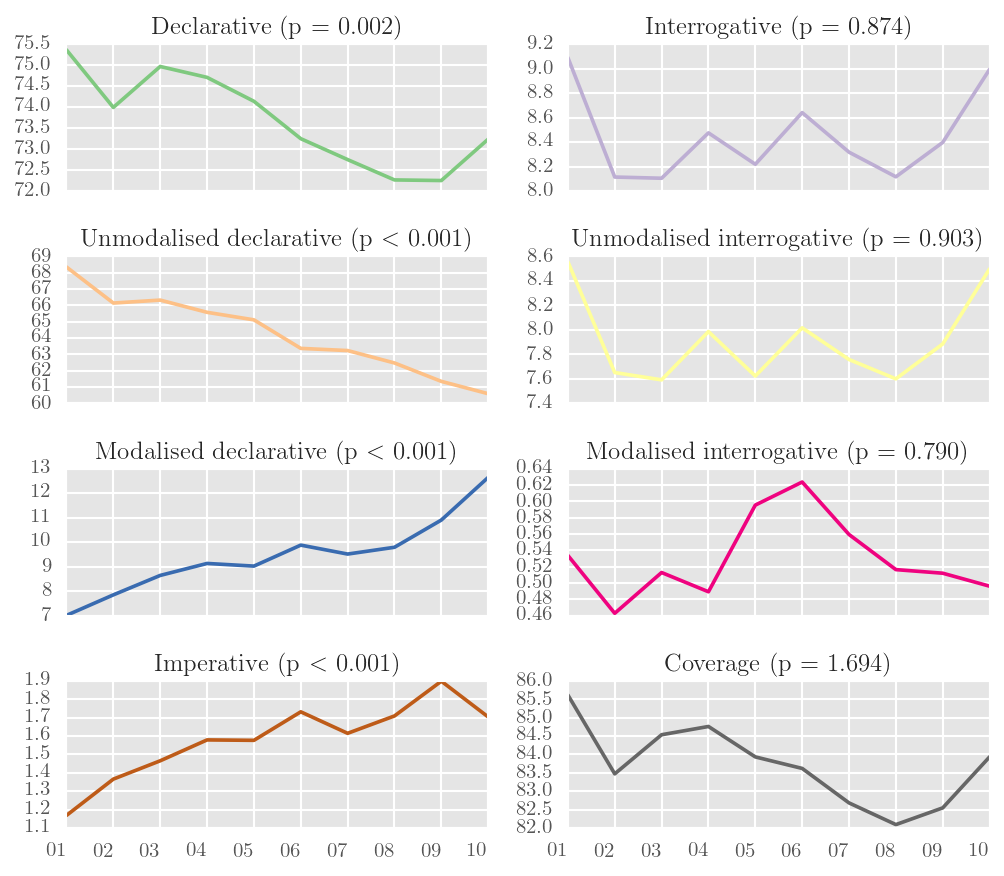
\includegraphics[width=0.8\textwidth]{../images/known-mood-and-indicative-types-in-p-corpus.png}
\caption{Mood features in the Membership Stage Structure}
\label{fig:mood_types_P}
\end{figure}

The broadest features of the \sctext{Mood} system that is reliably annotated by constituency parsing are the distinctions between Indicative and Mood Type (see Section \ref{sect:sfl}). Because dedicated tags for Mood Types are not available in either the constituency or dependency grammars, however, accurately locating them by automated searching alone is an unintuitive task. For this case study, \texttt{Tregex} expressions were developed, in order to discern major Mood and Indicative features from constituency parse trees (see Figure \ref{fig:mood_dict}). These queries must not just be designed for ideal, well\hyp{}formed cases, but must also handle false positives, such as sentence initial vocatives and salutations, which are often parsed as subject NPs. For interrogative matching, after many attempts to exploit Wh\hyp{}pronouns, Subject\hyp{}Finite order, it was determined that counting sentence final tokens containing at least one question mark was the most accurate method. When developing the constituency queries, accuracy was preferred over coverage. For this reason, only main clauses were analysed. To test the coverage of the queries, the total number of Mood Types found was compared to the total number of sentences (i.e. parse trees), minus any tree that did not contain a VP headed by a verb found in \texttt{VerbNet}. This removed a number of common, non\hyp{}major clausal parse trees, such as those provided for a minor clause like \emph{Hello!}.
%ntodo: verbnet reference?

\begin{table}
\centering
\footnotesize
\begin{tabular}{lrrrrr}
\toprule
{} &  Mod. declarative &  Unmod. declarative &  Interrogative &  Imperative &  Coverage \\
\midrule
$01$ &             $7.012$ &              $68.350$ &          $9.521$ &       $1.168$ &    $86.051$ \\
$02$ &             $7.849$ &              $66.143$ &          $8.618$ &       $1.366$ &    $83.976$ \\
$03$ &             $8.643$ &              $66.324$ &          $8.527$ &       $1.466$ &    $84.959$ \\
$04$ &             $9.132$ &              $65.576$ &          $8.967$ &       $1.579$ &    $85.254$ \\
$05$ &             $9.023$ &              $65.115$ &          $8.777$ &       $1.577$ &    $84.492$ \\
$06$ &             $9.880$ &              $63.367$ &          $9.183$ &       $1.732$ &    $84.163$ \\
$07$ &             $9.515$ &              $63.234$ &          $8.780$ &       $1.615$ &    $83.144$ \\
$08$ &             $9.792$ &              $62.474$ &          $8.640$ &       $1.710$ &    $82.616$ \\
$09$ &            $10.904$ &              $61.347$ &          $8.853$ &       $1.899$ &    $83.003$ \\
$10$ &            $12.645$ &              $60.592$ &          $9.283$ &       $1.704$ &    $84.224$ \\
\bottomrule
\end{tabular}
\caption{Relative frequency of Mood types}
\label{tab:mood_types_p}
\end{table}

The frequency of imperatives rises steadily through membership length (see Table \ref{tab:mood_types_p} and Figure \ref{fig:mood_types_P}), as veteran \glspl{member} may explicitly direct new \glspl{member} to do certain things: \emph{take care}, \emph{find the right meds}, or \emph{watch alcohol consumption}, for example, are common commands issued in veterans' \glspl{post}. Though advice given through imperatives provides suggested behaviour (as in the cases above), heavy grammatical constraints on the imperative mood (lack of Subject, tense, etc.) make elaboration within this kind of advice uncommon. Modality is also difficult to encode, as modal Finites cannot grammatically modify imperative Predicators (\emph{*Could go to the doctor}!). Imperatives thus rarely carry information regarding the addressee's level of obligation or the speaker's level of certainty or source of knowledge, and accordingly, can be face\hyp{}threatening for newcomers \cite{goldsmith2004communicating,hudson1990discourse}. For this reason, in veterans' \glspl{post}, unmodulated imperatives often function as general markers of social support (\emph{take care of yourself}; \emph{keep up the good work!}) rather than as suggested behaviour coupled with health information or marking of the source of the knowledge. Thus, there is no one-to-one relationship between the extent to which \gls{Forum} users make interactive demands on others and choices of Mood Type.

As shown in Table \ref{tab:mood_types_p}, declaratives shift over time, from unmodalised toward modalised type. This indicates a correlation between membership stage and the extent to which \glslink{member}{users} insert judgements of likelihood of propositions. This pattern can be interpreted as evidence of increasing social status over time. At the same time, however, the \sctext{Modality} system can be used as a resource for signalling incongruence between Speech Function and Mood Type (see the following section). Interrogatives, on the other hand, undergo no significant trajectory shift, as demonstrated in the significance calculations shown in Figure \ref{fig:mood_types_P}. Questions therefore comprise the same amount of talk at all stages of membership. As will be discussed below, while the overall frequency of the interrogative Mood remains stable, the kinds of propositions being negotiated in these questions undergo observable longitudinal change.

The calculation of \emph{Coverage} (Table \ref{tab:mood_types_p}\slash Figure \ref{fig:mood_types_P}) shows that the proportion of sentences for which Mood Type information could be obtained fluctuated, but in no clear direction. This increases confidence that observed changes in Mood Type proportions are not the result of consistent language changes that cause an increase or decrease in parser accuracy.

\section{Modalisation} \label{sect:modalisation}

Modalisation construes uncertainty within the clause as exchange. It is a more delicate feature of the \sctext{Mood} system than Mood Type, because its meaning changes depending on Mood selection: in declaratives, it congruently involves a speaker judgement; in interrogatives, it demands judgement from the addressee \cite{halliday_introduction_2004}. Different modal lemmata are responsible for communicating obligation, certainty, probability and usuality; at the same time, choices in modal lexis distinguish between low, median and high uncertainty, with negative and positive polarity at either pole (see Section \ref{sect:mood-grammar}: \sctext{Modality}).

%\begin{figure}[htb]
%\centering
%\includegraphics[width=0.6\textwidth]{../images/modals-when-subject-is-emphi.png}
%\caption{Mood features for the Membership Stage Structure}
%\label{fig:modalsb}
%\end{figure}
%
Over the course of membership, in general, Modalisation as a feature of Major clauses increases consistently (from 6.67\% to 8.83\% of all clauses). The major Mood Type accommodating this increase is the modalised declarative (Figure \ref{fig:mood_types_P}). A primary cause of this change is a strategy for advice provision that develops over the membership course. Rather than simply issuing commands with imperatives, much advice dispensed by veterans is realised by declaratives, generally featuring modalisation (see Figure \ref{fig:imp_and_mod} for examples). 

% modal examples
\begin{figure}
    %\minipage{0.44\textwidth}\centering
    \begin{tabular}[t]{@{}>{\raggedright\arraybackslash}p{0.45\textwidth}}
    \vspace{1mm}
    %\noindent\parbox[t]{0.44\textwidth}{\raggedright%
    \begin{enumerate} [before=\itshape,font=\normalfont] \setlength\itemsep{0em} \footnotesize
    %\item Keep talking and being patient ... it will happen but it isn't going to happen overnight like we all would like it too.
    \item Let us know how your appointments go!!
    \item Keep us posted with how things go.
    \item Keep on posting and let us know how you are doing.
    %\item Tell her what you just told us here... that you are not sleeping and that you knew that the wellbutrin was making you feel good with the mania but that you are afraid.
    %\item Make that call, Llama... you need to before this gets too out of hand and you are unable to know the difference.
    %\item Ask her if there is anything that you can do to make her feel better.
    %\item Get up and walk if you are able to for short periods of time... take your meds when you need to and a week after you feel better to cover things well.
    \item Try to pretend that you have a suit of armor on and try to allow as much of this to bounce off of you.
    \item Get a good night's sleep, eat right eliminating caffeine \& sugar from your diet, take your meds as prescribed, avoid stress as much as possible, get plenty of exercise and hold onto your sense of humor.
    \end{enumerate}
    \end{tabular}
    \begin{tabular}[t]{@{}>{\raggedright\arraybackslash}p{0.45\textwidth}@{}}
    
    \begin{enumerate}  [before=\itshape,font=\normalfont] \singlespacing \setlength\itemsep{0em} \footnotesize
    \item I would certainly make a point to follow up
    \item I would definitely have your daughter pay her
    \item I would highly recommend it
    \item I would DEFINITELY recommend seeing a psychologist
    \item I would definitely make mention of this
    \item I would strongly suggest that you discuss
    \item I would be very careful with just the Zoloft
    \item I would highly recommend that you take your meds on a daily basis.
    %\item I would also suggest you call NAMI.
    \end{enumerate}
    \end{tabular}
    %\endminipage
    \caption{Advice provision via imperatives and modalised declaratives}
    \label{fig:imp_and_mod}
    \end{figure}
    %
    \begin{figure}[htb]
    \centering
    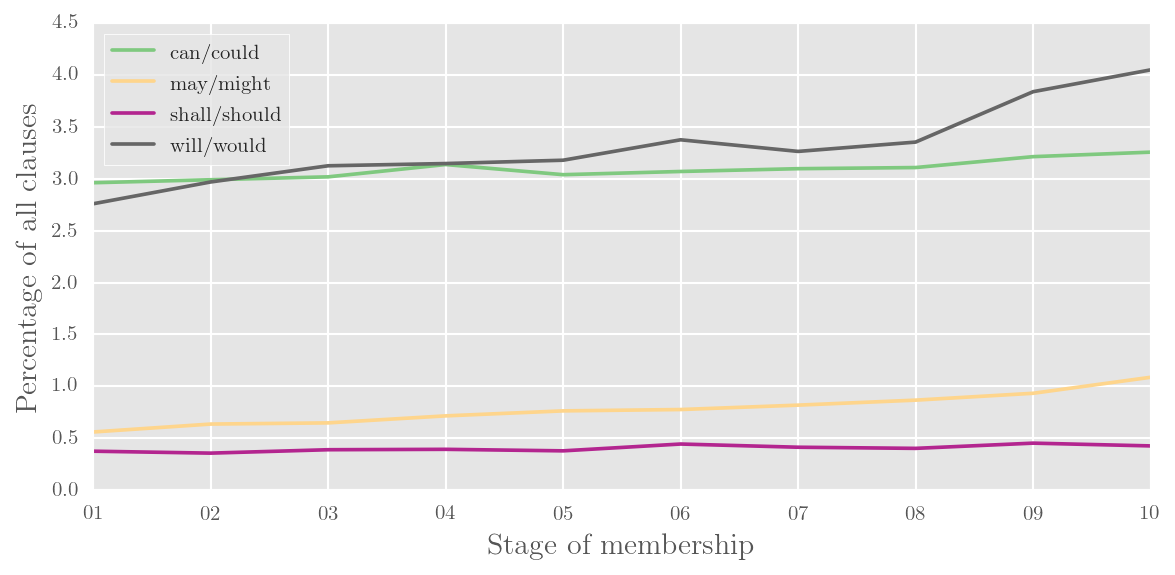
\includegraphics[width=0.6\textwidth]{../images/modalnew.png}
    \caption{Relative frequencies of modal lemmata}
    \label{fig:modals}
    \end{figure}
%
Figure \ref{fig:modals} shows that over the length of membership, there is a particularly marked increase in the frequency of \emph{would\slash will} modals, in comparison to other modal lemmata. Concordancing of declaratives modalised by \emph{would} was performed in order to understand their typical contexts of use. This revealed three things. First, veterans commonly dispense advice through hypothetical \emph{I would} statements (as in the examples above, and as seen in the qualitative analysis of Emz' post in Section \ref{sect:qual-reply-analysis}). Second, the modalised declarative is also often modulated by an Adjunct, in order to reconstitute perlocutionary force that was diminished through the incongruent selection of Mood Type (\emph{I would seriously\slash really\slash certainly consider quitting}). Third, the same grammatical construction also exists in new \gls{member} talk, but very rarely as a means of giving advice. Rather, \emph{I would (+ adjunct}) in first \glspl{post} often introduces a construal of past behaviour (\emph{I would get seriously drunk every night}---see Figure \ref{fig:vetmember_would} for contextualised examples).

%todo: split methods and findings a bit better?
As a result of this ambiguity, all \emph{I $+$ would $+$ adjunct} declaratives in new and veteran \glspl{member}' \glspl{post} (261\slash 143 total matches) were coded according to five inductively developed functional categories (outlined in Table \ref{tab:themcodes}). Three false positives (where \emph{'d} as a contraction of \emph{had} had been incorrectly parsed as a contracted \emph{would} modal) were excluded from analysis. The categories are not codified in the \gls{SFG}; rather, they are based on the apparent meaning potential of the register of \gls{Forum} talk. Categories are also not intended to be discrete: since a core purpose of modalisation is to express inclination, most instances of \emph{I would + adjunct} are on some level statements of inclination. Not all statements of inclination are descriptions of past behaviour, or provisions of advice, however.

%\emph{Will}-modalisation is also increasingly common over membership length. Issues of scope prevent its treatment here.}~

% 'jess' provides a future will modal in the qual analysis
   
% i would functions
\begin{table}[htb]
    \centering
    \footnotesize
    \begin{tabularx}{\textwidth}{p{2cm}XX}
    
    \toprule
    Category    & Description & Example       \\ \midrule
    Past Behaviour       & Habitual (generally negative) actions in the past   & \emph{And was around the time I would occassionally go to sleep for as much as 24 hours}     \\ 
    Advice       & Suggesting what another should do & \emph{I'd really encourage you to just call your psychologist back}    \\ 
    Request     & Requesting actions (typically information\slash support provision) from others      & \emph{I'd really appreciate any feedback from anyone on here}          \\
    Inclination and hypothetical & Preferences and inclinations, often in irrealis scenarios (within if-clauses) & \emph{I would never want to be without him; I wish I were sicker so that I wouldn't even worry about it} \\ 
    Hedged salutation            & Self introduction, explicit salutation      & \emph{I'm new here so I thought I'd just start out with a big ol' hi} \\ 
    Past sense of \emph{will}           & Talk of the future within narratives about the past---usually in Verbiage     & \emph{My father always told me that I would never mount to anything}   \\ \bottomrule
    \end{tabularx}
    \caption{Thematic categories of \emph{I would} + adjunct}
    \label{tab:themcodes}
    \end{table}
                    
    \begin{figure}[htb]
    \centering
    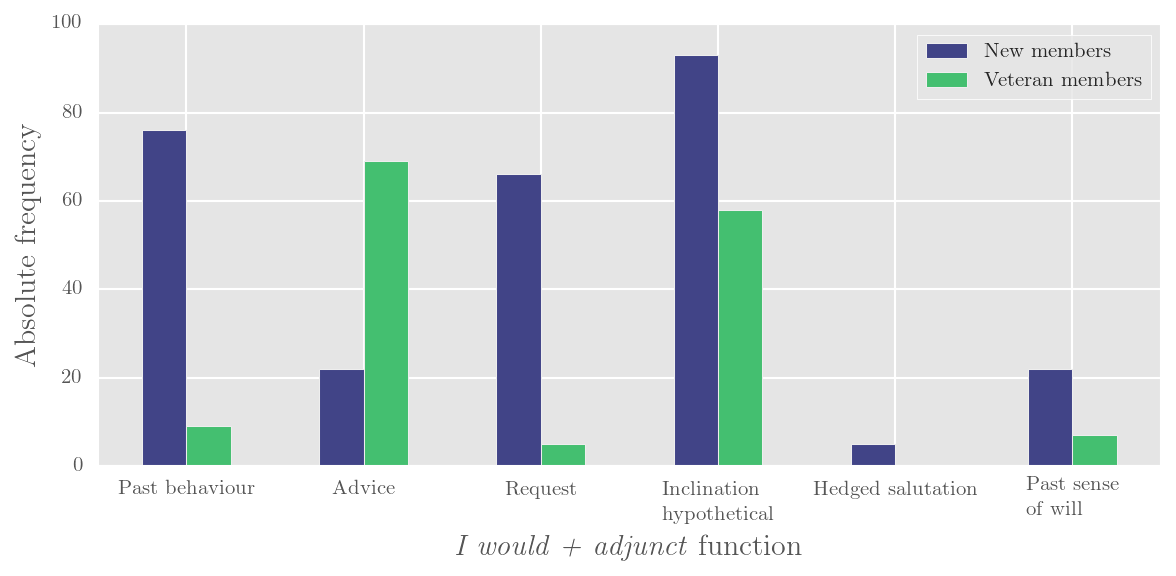
\includegraphics[width=0.75\textwidth]{../images/iwould-vid.png}
    \caption{Functions of \emph{`I would'} in new and veteran posts}
    \label{fig:i_would_func}
    \end{figure}
    
            %Concordancing \emph{would}-modalised declaratives in veteran posts revealed a distictive lexicogrammatical pattern for the provision of advice.
    
            %\enumsentence{\small{\emph{so many times i would walk over 40 km from my home to the city center, looking for people that didn't exist, at times i would even think beggars were spies ... or supernatural characters, very deluded and very weird ... many times i wouldn't sleep for at least 3 days, one time i didn't eat and sleep for 4 days !!!} (New member, post 1)}} % frokly
            %\enumsentence{\small{\emph{I would suggest that you go to the ER, explain your symptoms and then apply for assistance through a program like Medicaid} (Veteran member, post 1166)}} % dreamsinneon
    
                %\begin{figure}
                %  \centering
                %  \addvbuffer[12pt 8pt]{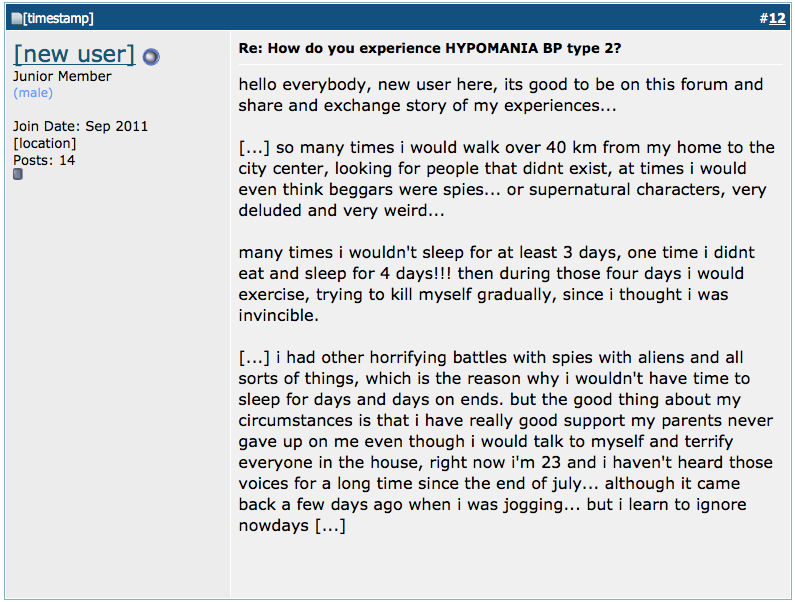
\includegraphics[width=0.65\textwidth]{../images/new_member_would.png}
                %  \caption{A new member's ``\emph{I would}'' construction}
                %               %\end{figure}
    
                %\begin{figure}
                %  \centering
                %  \addvbuffer[12pt 8pt]{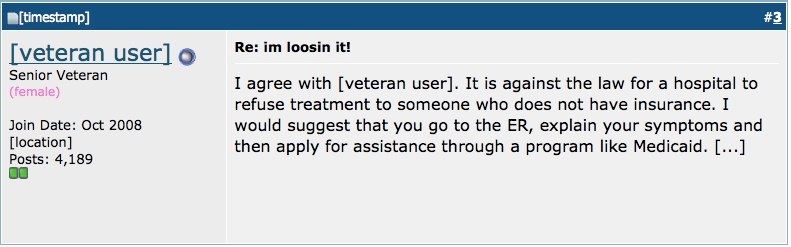
\includegraphics[width=0.65\textwidth]{../images/veteran_member_would.png}
                %  \caption{A veteran member's ``\emph{I would}'' construction}
                %  \label{fig:vetmember_would}
                %\end{figure}
    
Figure \ref{fig:i_would_func} shows that new and veteran members employ the \emph{I would + adjunct} construction for different purposes. In newcomer talk, it is commonly used to make incongruently realised requests (\emph{I would like to know ...}). This is a politeness strategy---veteran members seldom hedge their requests in this way. Also more common in newcomer talk are the uses of \emph{I would + adjunct} to index \emph{Past behaviour}, and as the \emph{Past sense of will}, an example of which can be found in Jess's first \gls{post} (\emph{i want to change my doctor and have been telling my partner i would}---see Section \ref{sect:jess-post}). From the perspective of genre, as highlighted in the previous Chapter, initial contributions conforming to generic structures include a substantial medical history, told in the past tense. For veterans, on the other hand, \emph{I would + adjunct} is predominantly used to signal advice. Aside from the general category of \emph{Inclination and hypothetical}, other functions are very uncommon in \glspl{post} made during the final stage of membership.

% The fact that manual analysis is necessary for such specific work highlights shortcomings in available \gls{NLP} tools. As such, when counting features, we must bear in mind that they may perform multiple functions. Chapter \ref{chap:futuredirections} discusses needed steps to automate this kind of categorisation.

%todo: is there a reference for this?
Advice realised by an \emph{I would} reveals much about the ways in which role relationships within the \glslink{Forum}{community} are discursively constructed. In contrast to health professionals' advice, \emph{I would} puts the veteran hypothetically in the position of the newcomer, highlighting their shared role as people living with \gls{bipolar}. At the same time, however, it stakes claim to higher social status: the construction implies not just a burden on the addressee to follow the advice, but also some more subtle social values---that veterans know more, and that the course of action they would personally take in such a situation is the right one. 

An experiential analysis of the \emph{I would} style of advice provision complements the interpersonal perspective here. The advice giver is construing him\slash herself experientially as the main participant in the figure, substituting the newcomer out of the construed reality entirely. This main participant is almost always an Agentive one: the most common processes include \emph{suggesting}, \emph{talking}, and \emph{going}. To emphasise agency further, veteran \glspl{member} may embed advice within a material process of \emph{going} (see Table \ref{tab:conc_iwould_action}), especially when the addressee is to be the Medium in the presented figure (\emph{I would go and get evaluated ...}). In turn, this emphasis on agency highlights for the addressee the need to take action in order to gain control over his\slash her health problems.

% conc: i would go and get ...
\begin{table}[htb]
\footnotesize
\begin{tabular}{rrl}

\toprule
        i wouldn't just &  go         &  and quit ... perhaps it is time to look for a less stressful job \\
                                        i'd &  go         &  right away and ask for major help from your pdoc \\
i would most definitely &  go         &  and be evaluated by a psychiatrist, that is absolutely the only way  \\
             n your shoes i would &  go         &  and get a second opinion from a doctor you've not been to before.              \\
                                     i would &  go         &  and get evaluated for bipolar if you thing that is what you have \\
and then i would &  go         &  talk with the pdoc and ask him why these meds .                                  \\
                      but i would definitely &  go         &  for that eval.                                                                  \\
\bottomrule
\end{tabular}
\caption{Emphasising action in veterans' advice to newcomers}
\label{tab:conc_iwould_action}
\end{table}
%
This foregrounding of subjective knowledge is very much at odds with Harvey's \citeyear{harvey_disclosures_2012} finding, where adolescents used a medicalised register to legitimate their claims. In the \glslink{Forum}{Bipolar Forum}, legitimacy is claimed explicitly through lay experience. While newcomers typically enter the \glslink{Forum}{community} with specific requests for information (about a side\hyp{}effect of a medication, or a problem with insurance, for example), veterans demonstrate an understanding of the illness course as a whole, with advice often taking into account a `bigger picture' that the newcomer is assumed to be not yet privy to. 

% examples of i would as html
\begin{figure}[htb]
\minipage{0.48\textwidth}\centering
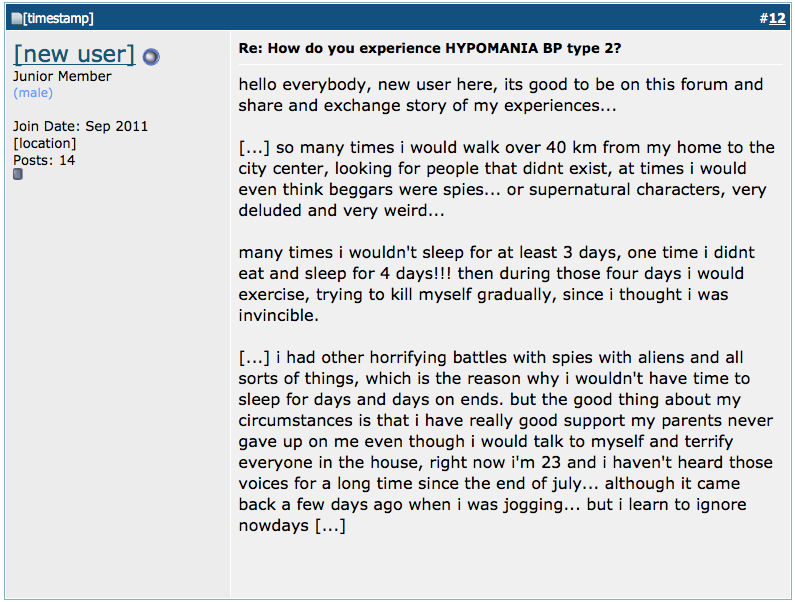
\includegraphics[width=1.00\textwidth]{../images/new_member_would.png}
\endminipage\hfill
\minipage{0.48\textwidth}\centering
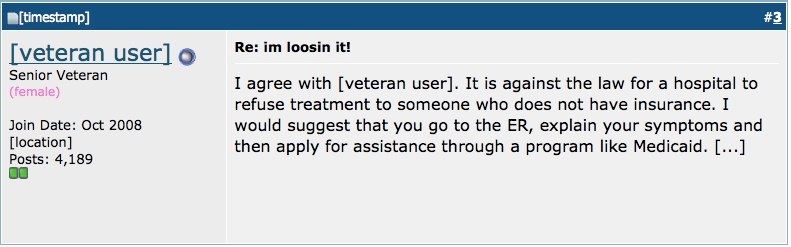
\includegraphics[width=1.00\textwidth]{../images/veteran_member_would.png}

\raggedright
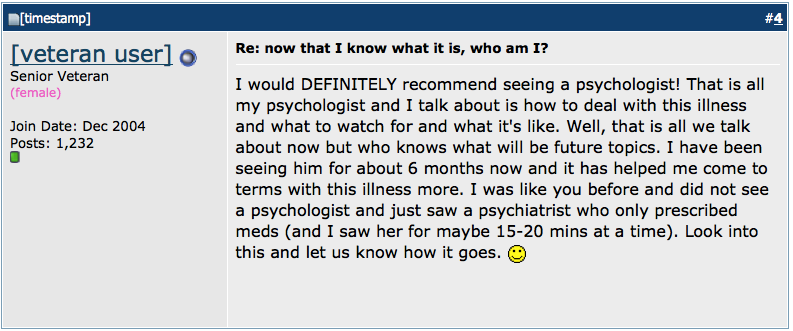
\includegraphics[width=1.01\textwidth]{../images/vet2would.png}

\endminipage\hfill
\caption[New and veteran members' `\emph{I would}' constructions]{Examples of typical new and veteran members' `\emph{I would}' constructions}
\label{fig:vetmember_would}
\end{figure}

%As the \glslink{Forum}{community} has a strong biomedical orientation, however, in which only health professionals can perform felicitous diagnosis, veteran members limit their advice to management through lifestyle choices, rather than medication regimens or new diagnoses.

%must mark their advice as grounded in lay-expertise. The issuance of imperative commands is a less common strategy than the use of incongruent modalised declarative commands. To reconstitute the force of the command, without overstepping the line that divides lay and professional kinds of health knowledge, veteran members employ adjuncts.

%The veteran's lay experiences---especially those experiences that occurred between his/her experience as a newcomer and the present moment---are construed as sufficient 

\FloatBarrier
\section{Mood elements}

In \gls{SFL}, the Finite grounds a proposition in time and space, making it \emph{arguable}. Arguability can be centred on primary tense, where propositions are debated with respect to when they occurred, in relation to the time of speaking. Alternatively, Modality can be argued. The Subject, meanwhile, is the thing charged with ensuring the carrying out of the proposition. By interrogating the \gls{corpus} for combinations of Subjects and Finites \cite[see][]{eggins_introduction_2004}, it is possible to chart change in who is made responsible, in the clause\hyp{}as\hyp{}exchange.

% Pronoun-Subject + Modal-Finite blocks as a percentage of all clauses in the P Corpus
\begin{figure}
    \centering
    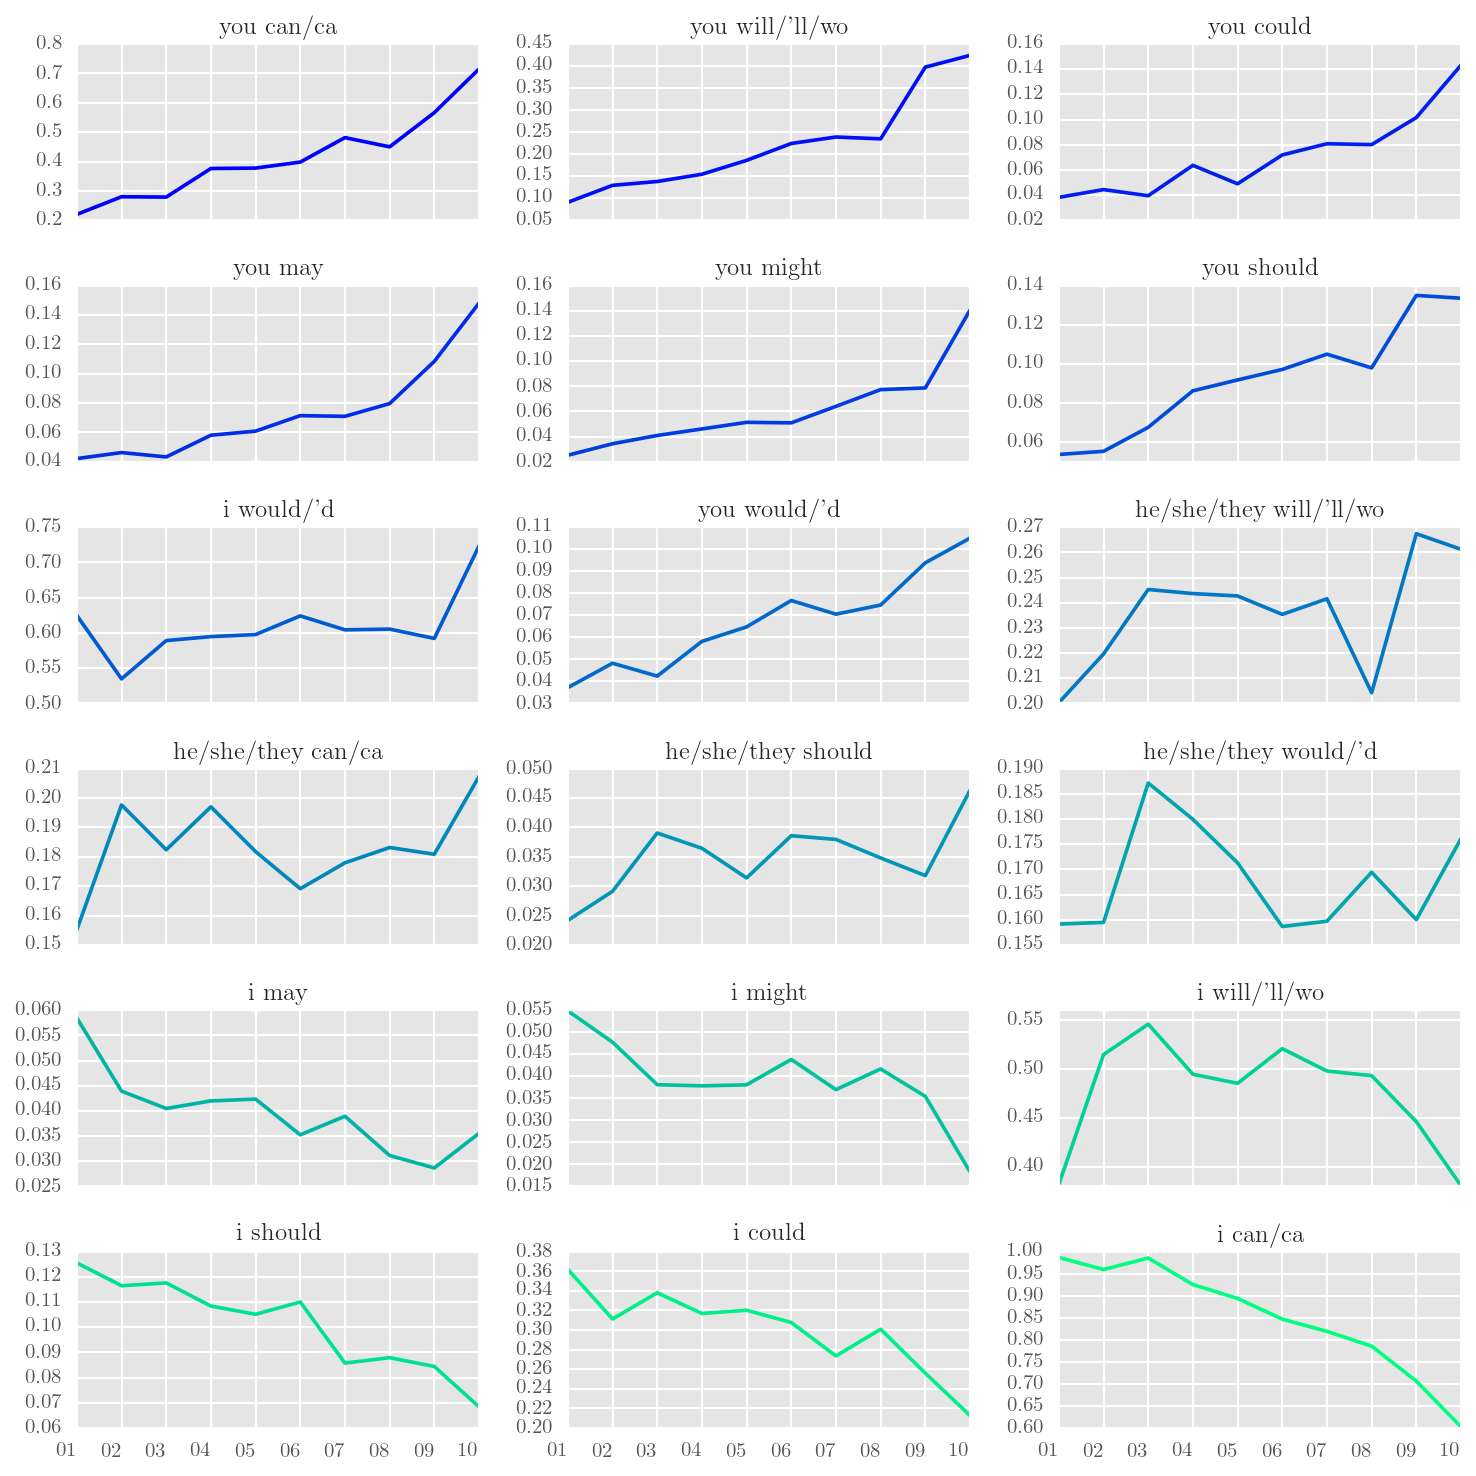
\includegraphics[width=1\textwidth]{../images/subj-fin-const-p-page.png}
    \caption[Pronoun-Subject + Modal-Finite blocks]{Pronoun-Subject + Modal-Finite blocks as a percentage of all clauses}
    \label{fig:modal_constellations}
    \end{figure}%
%
The frequencies and trajectories of configurations of Pronominal subjects and modal Finites can be used to determine the kinds of proposals and propositions being debated. Figure \ref{fig:modal_constellations} shows that generally, \emph{I $+$ modal} is displaced by \emph{you $+$ modal} over the course of membership. In fact, \emph{I would} stands out as the only \emph{first person $+$ modal} block on an increasing trajectory. This is due to its frequent use as a means of giving advice, as discussed above. Though modals negotiate a diverse range of concepts, such as certainty, probability and obligation, the \emph{Subject $+$ modal} configuration still places an interpersonal burden on the Subject as the one charged with bringing the Predicator about. Accordingly, newcomers self\hyp{}assign the burden, while veteran members turn to direct interpersonal demands on their interlocutors. This is not to say, of course, that the veteran\slash newcomer relationship is one that mistreats the newcomer. The dynamic is a symbiotic one. Veteran membership comes with a kind of expertise, which is being exchanged with other \glslink{Forum}{community} members through advice. Veterans answer others by explaining what is possible, feasible, likely or uncertain.

Mood Blocks can also be viewed through the lens of \glslink{Forum}{community} membership conditions. In early \glspl{post}, \glslink{member}{users} narrate their medical history, setting out credentials for acceptance by the user base. Veteran \glspl{member} act as interviewers, requesting further information, or grafting the presented narratives to the community's normative biomedical ideology. Newcomers are under observation, and are expected to assist in veterans' assessments by providing a narrative account of their illness course. This is particularly important in first \glspl{post}, but extends generally to cover early contributions, in which the new user is primarily focussed on the self.

Figure \ref{fig:modal_constellations} also shows that the trajectory of \emph{third person $+$ modal} constructions is generally inconsistent or stable. This is because role\hyp{}relationship negotiation is carried out by making or fulfilling the demands of interlocutors, rather than things and people being spoken about. There is therefore little difference over the course of membership in the way non\hyp{}present participants are modalised. Rather, as we will see later, non\hyp{}present participants undergo a number of changes within the system of \sctext{Transitivity}.

Of all constellations, \emph{I $+$ can} (and its derivatives and interrogative inversion) undergoes the most radical change. In a question, this kind of Mood Block expressly asks others for information or permission. As can be seen in Table \ref{tab:conc_i_can_first}, in first \glspl{post}, in declarative form, \emph{I can} is very often negated, with contributors narrating difficulties carrying out healthy mental processes (\emph{cope, focus, make up mind, handle\slash stand it, stand it, remember own name, have no emotion, feel normal}), controlling harmful behavioural processes (\emph{can't stop crying, can barely stay awake, can't breathe}), and performing vague material processes (\emph{get things done, nothing I can do about it, get out of everyday life}). Over the membership course, the construction falls into disuse: unlike \emph{I would}, it is very rarely employed as a proposal (e.g. \emph{I can PM you this if you like}).

% Concordancing \emph{I can} mood blocks in first \glspl{post}
\begin{table}[htb]
    \footnotesize
    \begin{tabular}{lrl}
    \toprule
    0  &  antly stressed , i had migranes and &  i could n't sleep , i could n't go out for to long be\\
    1  &  ad migranes and i could n't sleep , &  i could n't go out for to long because i just always \\
    2  &  s just started to get abit better , &  i could go out again                                 \\
    3  &  nd i did want to end it all because &  i could n't take the fear anymore                    \\
    4  &              i ' v also noticed that &  i can get really angry , really easily these days too\\
    5  &   - if anyone has any tips about how &  i can lose weight and not gain anymore whilst on depa\\
    6  &  st but i 've coped with it the best &  i can                                                \\
    7  &     i~'m not working right now , but &  i ca n't seem to get anything done around my house   \\
    8  &  t have tutors come to my house when &  i could handle them                                  \\
    9  &  f out of bed in the morning and all &  i can think about all day                            \\
    10 &                                      &  i can not stop crying .                              \\
    11 &                                      &  i can barely stay awake .                            \\
    12 &   i feel so fat and disgusting , but &  i ca n't stop eating                                 \\
    13 &                          i just wish &  i could make them feel how i 'm feeling , just so the\\
    14 &  al and i feel like there 's nothing &  i can do about it                                    \\
    15 &  erally just keep thinking about how &  i can go back to the psych ward                      \\
    16 &  go back to the psych ward , just so &  i can get out of everyday life for a while           \\
    17 &                                      &  i can not get along with any of my coworkers , as wel\\
    18 &                                      &  i ca n't process any of my rapid thoughts and have ju\\
    19 &                                      &  i ca n't think of any reason why this occurs and do n\\
    \bottomrule
    \end{tabular}
    \caption[Concordancing \emph{I $+$ can} Mood Blocks]{Concordancing \emph{I $+$ can} Mood Blocks in first \glspl{post}}
    \label{tab:conc_i_can_first}
    \end{table}
%
This pattern can also be approached in terms of membership entry conditions. Newcomers often stress the seriousness or urgency of their case, based on the existence of some ongoing mental or physical harm.

\subsection{Tense}
%todo: the two figures presented here get reversed due to size, which i don't like

\FloatBarrier

If not by \sctext{Modality}, arguability happens along the lines of \sctext{Tense}---the relationship between a proposition and the time of speaking. Figure \ref{fig:tense_constellations} shows different configurations of pronominal Subject and Tense. More specifically, it shows that tense of modals is not a feature that exhibits consistent change over time: the trajectory shifts are caused for the most part by changing frequencies of pronominal Subject choice.

% Tense of tensed clauses over the course of membership
\begin{figure}[htb]
\centering
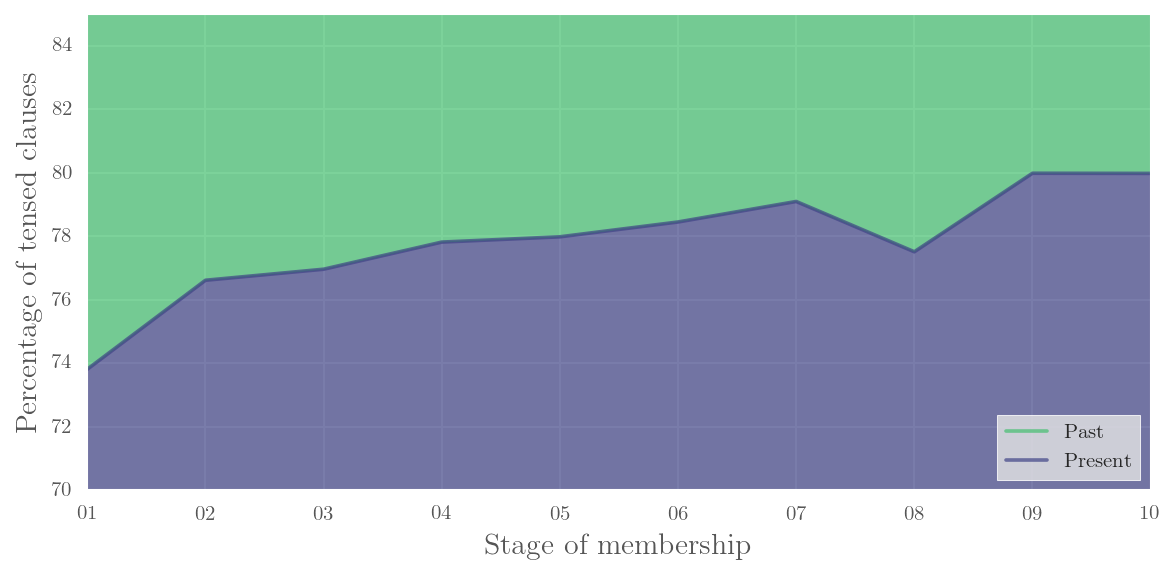
\includegraphics[width=.7\textwidth]{../images/tense-area.png}
\caption{Tense of tensed clauses over the course of membership}
\label{fig:tense-area}
\end{figure}
%
The system of \sctext{Tense} can be isolated from its co\hyp{}text, however. Figure \ref{fig:tense-area} plots primary tenses of non\hyp{}modalised clauses over the membership course. The steady transition from past toward present (from 74 to 80 per cent of all tensed clauses) demonstrates a shifting focus from setting out medical history narratives as membership credentials to helping others with their current problems. At an ideological level, the shift also represents a gradual refocussing on present and future actions, both of the self and of addressees.

% Pronoun-Subject + Past\slash Present tense blocks as a percentage of all Major clauses in the P Corpus
\begin{figure}[htb]
\centering
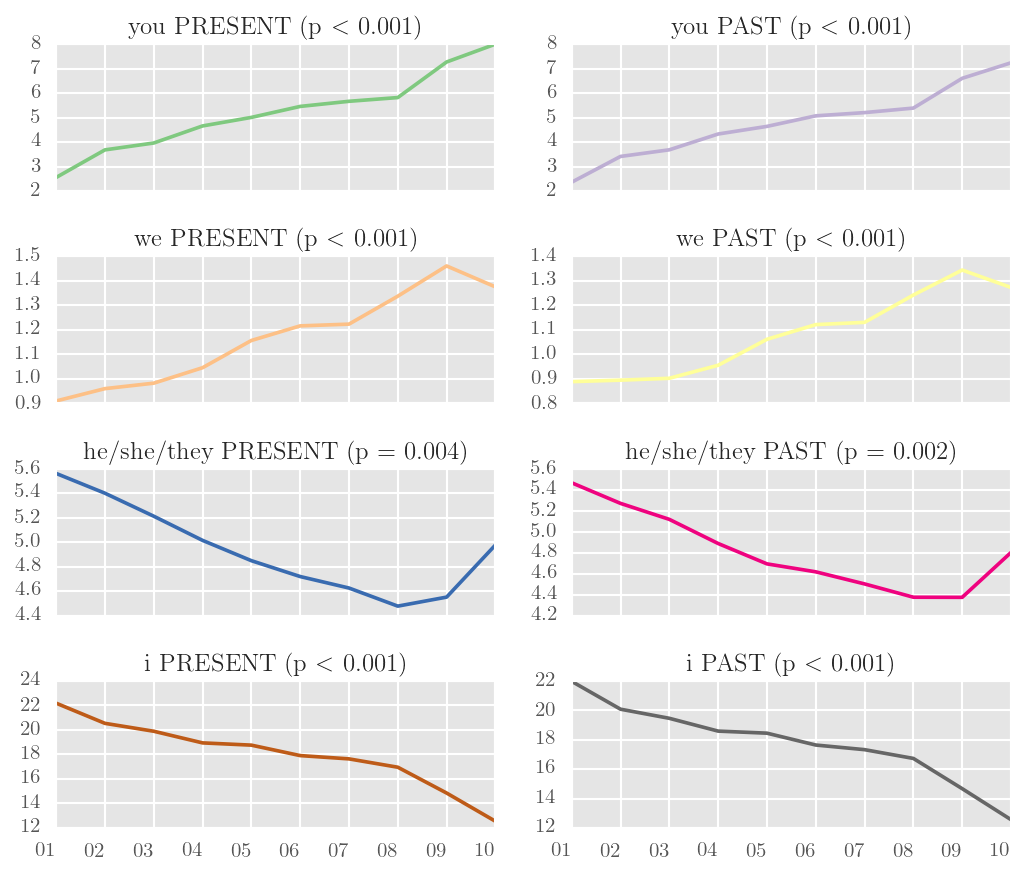
\includegraphics[width=1\textwidth]{../images/subj-ten-const-p.png}
\caption[Pronoun-Subject + Past\slash Present tense blocks]{Pronoun-Subject + Past\slash Present tense blocks as a percentage of all Major clauses for the Membership Stage Structure}
\label{fig:tense_constellations}
\end{figure}

\subsection{Polarity}

The final component of the interpersonal analysis is the system of \sctext{Polarity}.\endnote{There was little reason to expect dramatic or consistent polarity shifts over the course of membership. The analysis is carried out and presented mostly for the purposes of completeness of the register description.}~Clauses may have positive or negative polarity. The default polarity is positive; negative polarity is realised through a small group of lexical items (\emph{n't\slash not}, \emph{no}, \emph{never}) that appear in close proximity, or fused with, the Finite. Therefore, polarity can be interrogated using \texttt{Tregex} queries:

\begin{verbatim}
Negative = 'VP !> VP <+(VP) (VP !< VP <<# (/VB.?/ < /$VERBLIST/)) \
           ' <<# /(VB.?|MD)/ < (RB < /(?i)^(n.t|never|no)$/)'
Positive = 'VP !> VP <+(VP) (VP !< VP <<# (/VB.?/ < /$VERBLIST/)) \
           ' <<# /(VB.?|MD)/ !< (RB < /(?i)^(n.t|never|no)$/)'
\end{verbatim}

\begin{figure}[htb]
    \centering
    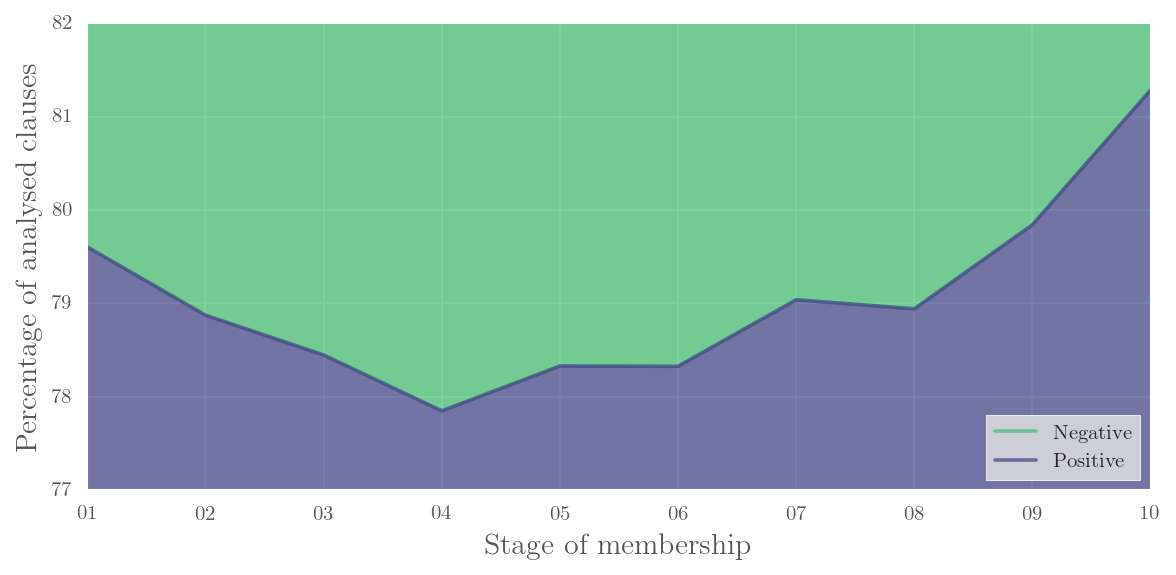
\includegraphics[width=.7\textwidth]{../images/polarity-area.png}
    \caption{Clause polarity over the course of membership}
    \label{fig:polarity}
    \end{figure}

\sctext{Polarity} figures into other places within interactions, such as as minimal responses to polar interrogatives. These kinds of minor clauses are not considered here; only clauses containing a verb\hyp{}form in \texttt{WordNet} are considered. Figure \ref{fig:polarity} shows that clause\hyp{}level polarity choices have an unstable trajectory over the membership course, decreasing until the 8--15th post, and then increasing. The fact that this result is difficult to interpret is unsurprising: the meaning of polarity is to some extent dependent on Mood Type, and on the previous move in the exchange. Moreover, unlike a linguistic feature like passivisation or grammatical metaphor, the ratio of positive\slash negative polarity clauses does not have a direct or clear relationship with \glspl{discourse-semantic} within a clause, except perhaps in a few rare cases (i.e. a list of rules). As noted in Section \ref{sect:mood-grammar}, \sctext{Polarity} is more likely to provide insights into discourse when examining entire interactions, rather than individual \glspl{post}. Even so, one point of note is that negative polarity is approximately twice as frequent as the ratio (ten per cent of all clauses) suggested by \textcite{halliday_introduction_2004}.

It is also possible to search for polarity in combination with other Mood features, in order to determine whether combinations of Modality $+$ Polarity, or Pronominal Subject $+$ Polarity, are undergoing change. In Figure \ref{fig:subjmodpol}, modals are grouped into four types. Distinctions are also made between first and second person Subjects, and between positive and negative polarity. Again, this kind of analysis shows, when compared to choices of Subject and modal, polarity choices play only a minor role in the longitudinal register shift of \glspl{member} of the \glslink{Forum}{Bipolar Forum}.

% subj mod pol
\begin{figure}[htb]
    \centering
    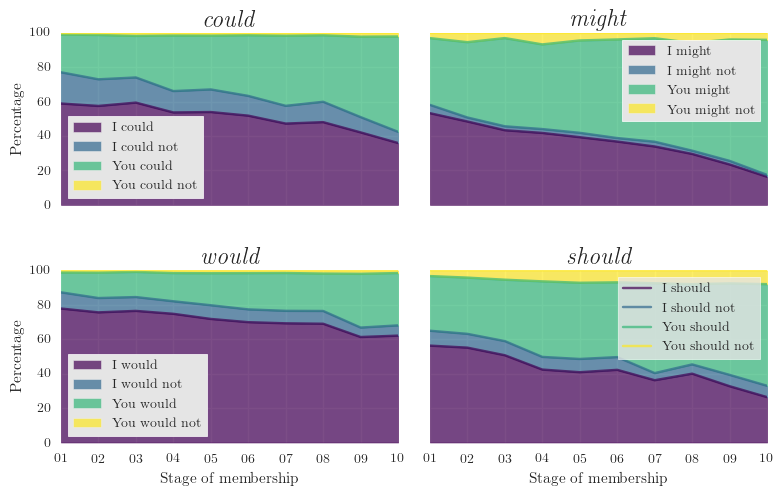
\includegraphics[width=.8\textwidth]{../images/subjmodpol.png}
    \caption{Constellations of Subject, Modal and Polarity}
    \label{fig:subjmodpol}
    \end{figure}
% analysis

\section{Summary}

Mood and Indicative Types shift across the course of membership: imperatives and modalised declaratives become more frequent as users gain the social capital necessary to dispense advice or make (semiotic) demands on newcomers. Interrogatives do not exhibit a clear trajectory, because the \glslink{Forum}{community} roles of both veterans and newcomers involve asking questions. For newcomers, questions are a means of obtaining information from the longer\hyp{}term users; for veterans, questions are used to elicit information that may aid in advice provision. Questions can be used to demonstrate interest and investment in the narratives of others, and to hold others accountable for perceived absences from the group (\emph{Where did ya go?}); alternatively, they can be used to invite newcomers to return to the community and\slash or to contribute again \cite{paulus_`please_2015}.

%todo copy edit
\sctext{Modality} is used throughout membership, with increases in later stages. Exploration of \emph{I $+$ would} clauses reveals shifts in the socio\hyp{}semantic activities in which \gls{Forum} members engage, from narration of past circumstances (\emph{sharing}) toward hypotheticals and suggestions for further behaviour \cite[\emph{advising}---see][]{matthiessen_applying_2013,matthiessen_modeling_2015}. This, however, is a registerial insight that blends components of Field and Tenor \cite{Matthiessen2015}. Looking at Mood Blocks more generally, a clear transition takes place over the course of membership: new and veteran members alike co\hyp{}operate to hold the less senior \glspl{member} modally responsible in discourse. The system of \sctext{Tense} exhibits change when modal tense is excluded, showing a longitudinal orientation toward the present and future, away from the past. \sctext{Polarity} is shown to vary inconsistently when analysing \glspl{post} alone, and to generally play a subordinate role to other components in the \sctext{Mood} system.

In the next chapter, I use dependency parses to investigate longitudinal changes in experiential meanings made in the \gls{Forum}, via choices of \sctext{Transitivity}.
